\section{Experiments}

In this section, we provide a comprehensive empirical evaluation of ARMOR.
We first present the main results across different base models and RL algorithms to validate the framework's broad effectiveness in mitigating over-optimization. 
Subsequently, we conduct detailed ablation studies to dissect the individual contributions of the two core components in ARMOR, as well as the impact of various reference policy settings.

\subsection{Main Results}

\textbf{Experimental Setup}.
To verify that ARMOR effectively addresses the over-optimization problem, we adopt the \textbf{continual training} setting described in Section~\ref{sec:kl}.
We employ two base models: Qwen2.5-Math-7B \citep{Qwen25Math} and Qwen3-8B-Base \citep{Qwen3}, trained on the DAPO-Math-17K dataset.
For the underlying RL algorithms, we select DAPO \citep{DAPO} and QAE \citep{QAE}. 
QAE represents a state-of-the-art method with a quantile-based advantage function, which we integrate into our framework by replacing the advantage term in Eq.~\eqref{eqn:advantage}.

The training protocol proceeds in two stages: we first run the baseline algorithm until validation performance degrades due to over-optimization. 
We then apply ARMOR to continue training from the best checkpoint (identified via the AIME24 validation set) prior to performance collapse. 
Detailed experimental setting and hyperparameters are provided in Appendix~\ref{appendix:impl}.

\textbf{Benchmarks and Metrics}. 
We evaluate performance on both mathematical reasoning and general capabilities. 
For reasoning, we report both the average accuracy (\texttt{avg@k}) and \texttt{pass@k} \citep{passk} on challenging mathematical benchmarks, including AIME24/25 and AMC. 
We also evaluate the model's general capabilities on science reasoning \citep[GPQA,][]{GPQA} and language understanding \citep[MMLU-Pro,][]{MMLU-Pro}. 
For math reasoning tasks, we sample 32 responses to derive a robust estimation. 
For general tasks, we use 8 samples due to the significantly larger query volume. 
All reported checkpoints are selected based on their AIME24 performance.

\begin{figure*}[t]
    \centering
    \begin{subfigure}[b]{0.325\linewidth}
        \centering
        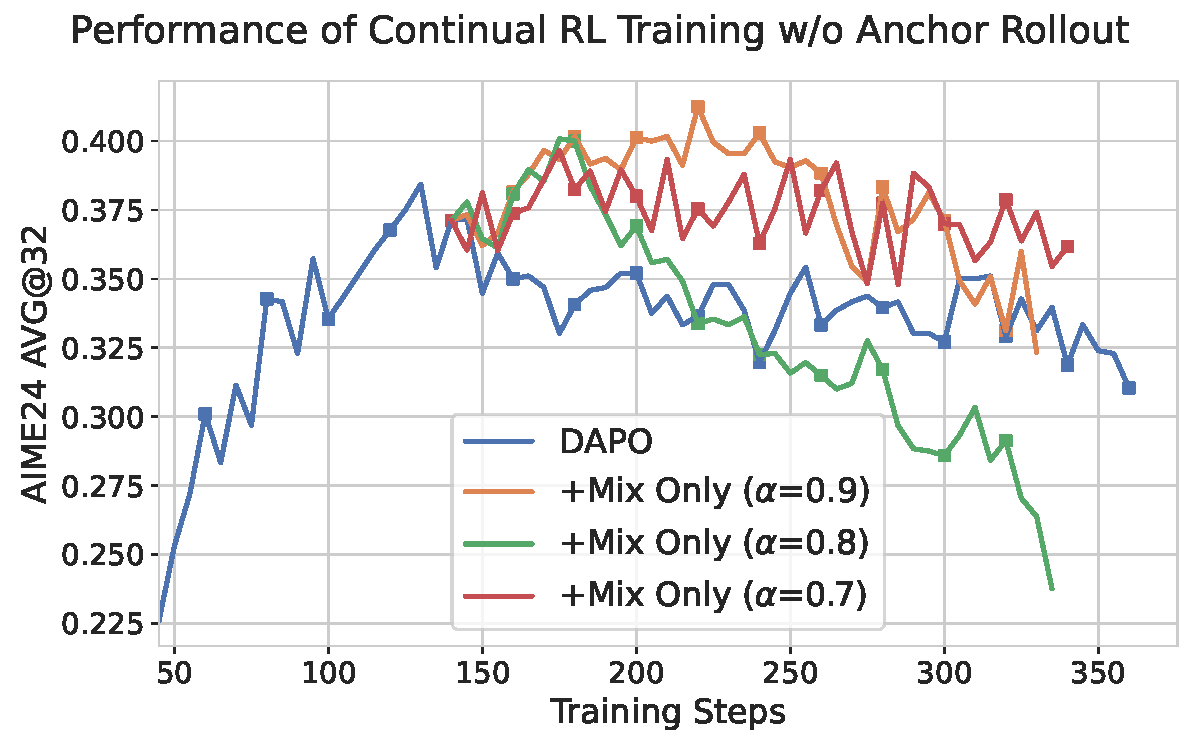
\includegraphics[width=\linewidth]{figs/mix_only.pdf}
        \caption{Without Anchor Rollout}
        \label{fig:no_anchor}
    \end{subfigure}
    \hfill
    \begin{subfigure}[b]{0.325\linewidth}
        \centering
        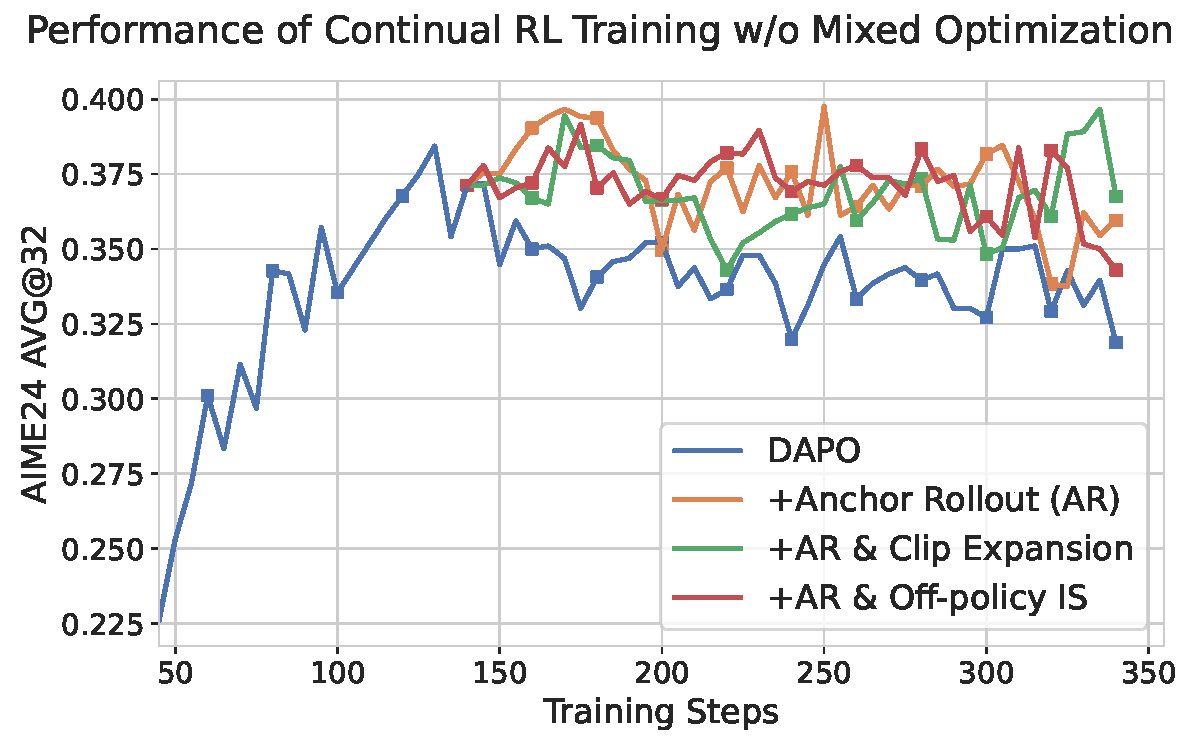
\includegraphics[width=\linewidth]{figs/is_ablation.pdf}
        \caption{Without Mixed Optimization}
        \label{fig:no_mixed}
    \end{subfigure}
    \hfill
    \begin{subfigure}[b]{0.325\linewidth}
        \centering
        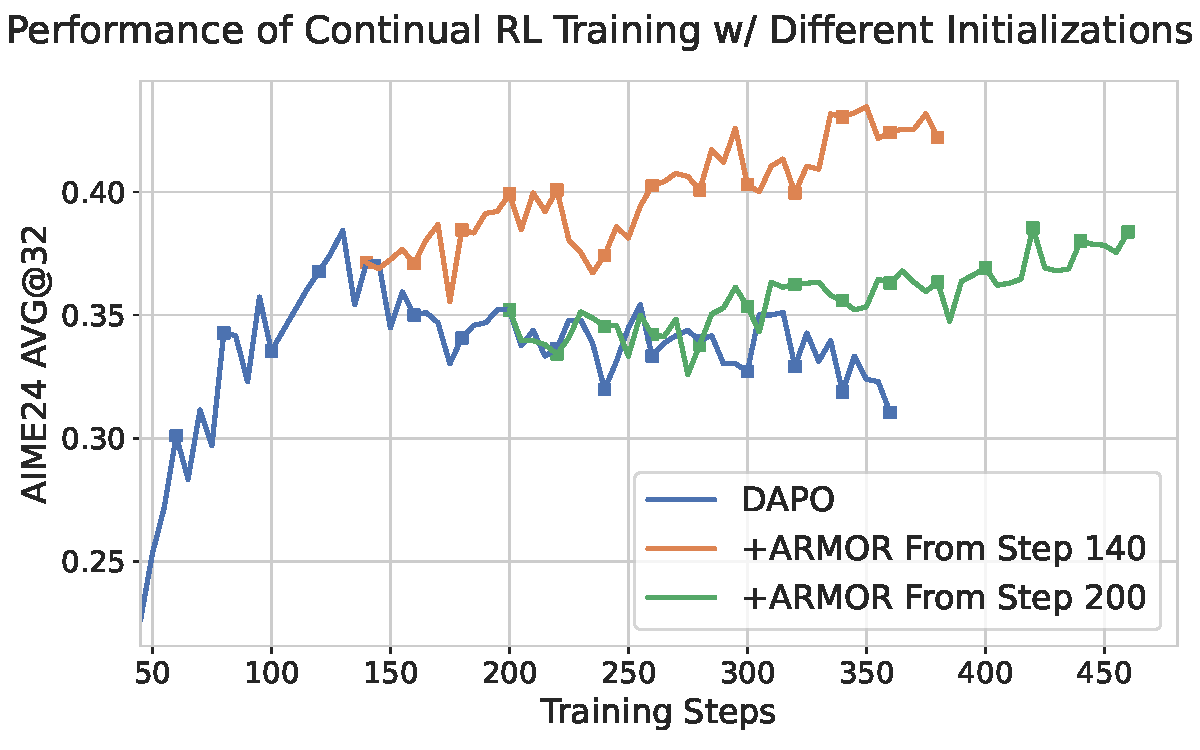
\includegraphics[width=\linewidth]{figs/different_restart.pdf}
        \caption{Robustness to Initial Model Quality}
        \label{fig:diff_start}
    \end{subfigure}
    \caption{(a) \textbf{Necessity of Anchor Rollout}. 
    We compare \textcolor{myblue}{DAPO} against variants using \emph{only} Mixed Optimization ($\alpha$ = \textcolor{myorange}{0.9}, \textcolor{mygreen}{0.8}, and \textcolor{myred}{0.7}).
    Without the stability foundation provided by Anchor Rollout, these models suffer from eventual performance collapse.
    (b) \textbf{Necessity of Mixed Optimization}.
    We replace mixed optimization with alternative objectives on top of Anchor Rollout (AR).
    While \textcolor{myorange}{AR alone} effectively stabilizes training, modifying standard objectives with \textcolor{mygreen}{comparable clip range} or \textcolor{myred}{off-policy IS} fails to yield further improvements.
    (c) \textbf{Ablation of different initializations}.
    We apply ARMOR to models initialized from an optimal checkpoint \textcolor{myorange}{(Step 140)} versus a collapsed checkpoint \textcolor{mygreen}{(Step 200)}. 
    Remarkably, ARMOR successfully recovers performance even from a degraded state, although initiating from a higher-quality model enables a higher final performance peak.
    }
\end{figure*}

\textbf{Performance Analysis}.
As summarized in Tab.~\ref{tab:main}, while standard training suffers from over-optimization (so the select checkpoints undergo fewer training steps), ARMOR successfully stabilizes the training process and secures sustained performance gains beyond the initial peak:
\begin{itemize}[left=0em,topsep=0pt,itemsep=0pt]
    \item \textbf{Significant Gains with DAPO:} On both Qwen2.5 and Qwen3 variants, applying ARMOR to DAPO yields substantial improvements, boosting average math scores by \textbf{+5--8 points}. Notably, this reasoning gain does not come at the expense of general capabilities, which also see clear enhancement by \textbf{+2--6 points}.
    \item \textbf{Robustness with QAE:} When applied to QAE, ARMOR further improves mathematical reasoning by \textbf{+1.7 points}, validating its robustness across different algorithms.
    While we observe a slight regression in general capabilities, we attribute this to two factors: the extended training horizon naturally increases the risk of forgetting for general knowledge, and more importantly, QAE's advantage masking mechanism\footnote{QAE uses reward quantiles as an advantage baseline, naturally producing zero-advantage samples (typically $\sim$80\% of the batch).} can inadvertently discard our injected anchor samples $y_\text{anc}$, thereby weakening the regularization effect (We also observe a larger $\mathbb D_\text{KL}(\pi_\text{ref}\|\pi_\theta)$ than DAPO's in our experiments).
\end{itemize}
Overall, ARMOR consistently extends the effective training window and pushes the reasoning performance ceiling across all tested settings.
As a two-stage recipe, ARMOR also outperforms teacher-guided OPD~\citep{agarwal2024policy} and MOPD~\citep{xiao2026mimo} baselines initialized from the same best zero-RL checkpoint (Appendix~\ref{appendix:two_stage}).
% Beyond directly continuing RL, we also consider a broader view of \emph{two-stage} training: using the best zero-RL checkpoint as a teacher policy for the second stage.
% We instantiate this setting with representative recipes such as OPD~\citep{agarwal2024policy} and MOPD~\citep{xiao2026mimo}, and report the comparison in Appendix~\ref{appendix:two_stage}, where ARMOR consistently outperforms these baselines.


\begin{table}[t]
\centering
\caption{
\texttt{Pass@k} evaluation of ARMOR compared to baselines. 
The checkpoints used for evaluation are consistent with Table~\ref{tab:main}. 
ARMOR maintains or improves \texttt{pass@16} despite extended training horizons, indicating robust intrinsic reasoning improvements.
}
\label{tab:passk}
\resizebox{\linewidth}{!}{
\begin{tabular}{@{}ccccc@{}}
\toprule
\textbf{} & \textbf{AIME24} & \textbf{AIME25} & \textbf{AMC} & \textbf{Average} \\ \midrule
7B-DAPO & 55.75 & 34.96 & 90.82 & 60.51 \\
\textbf{+ARMOR} & 56.52 & 39.44 & 90.89 & \textbf{62.28} \\ \midrule
7B-QAE & 51.21 & 30.71 & 88.52 & 56.81 \\
\textbf{+ARMOR} & 50.33 & 34.08 & 86.12 & \textbf{56.84} \\ \midrule
8B-DAPO & 70.65 & 50.88 & 90.24 & 70.59 \\
\textbf{+ARMOR} & 74.60 & 51.42 & 90.66 & \textbf{72.23} \\ \bottomrule
\end{tabular}
}
\end{table}

\textbf{\texttt{Pass@k} Evaluation}.
Beyond average performance, we investigate intrinsic reasoning capability via the \texttt{pass@k} metric \cite{yue2025does}.
Tab.~\ref{tab:passk} reports \texttt{pass@16} results on three math benchmarks \citep{passk}. 
ARMOR achieves comparable or improved scores across all models and baselines, confirming that our method effectively raises the model's absolute problem-solving ceiling rather than simply trading off \texttt{pass@k} for accuracy.

\vspace{-3pt}
\subsection{Ablation Study}
To understand the source of ARMOR's gains, we dissect the framework to analyze the necessity of Anchor Rollout, Mixed Optimization, and the impact of reference policy.
% To understand the source of ARMOR's gains, we dissect the framework to individually analyze the necessity of Anchor Rollout, Mixed Optimization, and the impact of different reference policy settings.

\begin{figure*}[t]
    \centering
    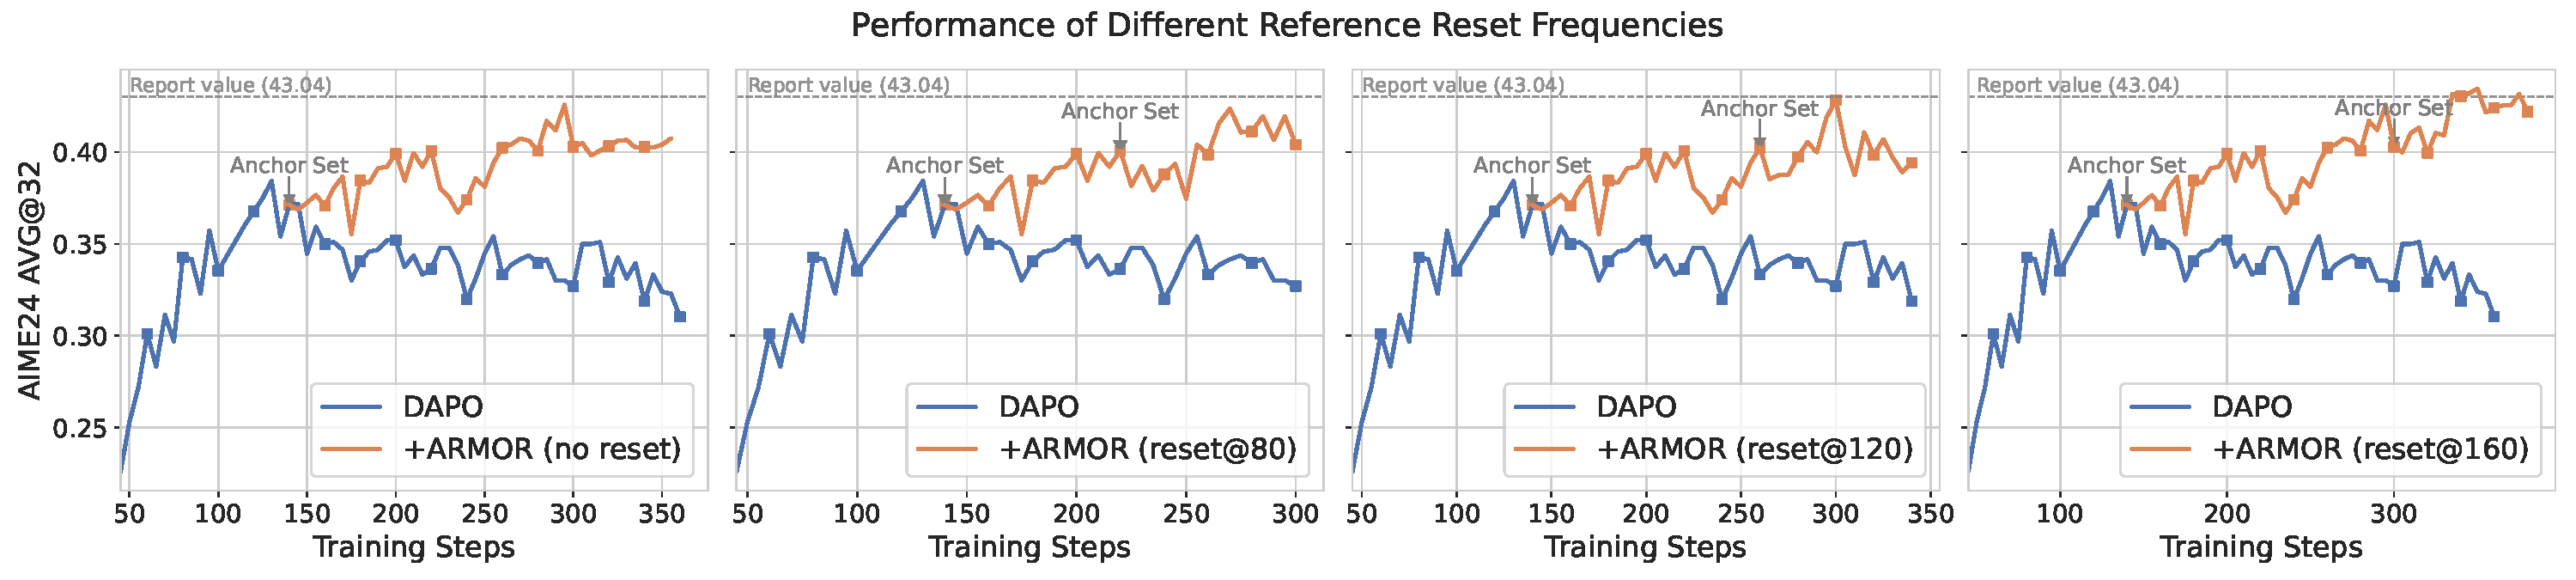
\includegraphics[width=\linewidth]{figs/different_reset.pdf}
    \caption{\textbf{Impact of Reference Reset Frequency.} 
    We compare ARMOR training with a static anchor (no reset) versus resetting the reference policy every 80, 120, or 160 steps (noted by ``Anchor Set'' in the figure).
    Periodic resets allows the anchor to evolve with the policy, preventing stagnation and fostering higher reasoning accuracy.}
    \label{fig:diff_reset}
\end{figure*}

\vspace{-3pt}
\subsubsection{Necessity of Anchor Rollout}
We first test a variant using only Mixed Optimization (Eq.~\ref{eqn:mixed_is}) without injecting anchor samples, so the only difference from DAPO here is the replaced IS ratio: $r_{i,t}^\text{mix}$.
As shown in Fig.~\ref{fig:no_anchor}, on the one hand, this variant can achieve initial growth across different mixing coefficients $\alpha$, with the peak performance increased from 37 to 40+, showcasing Mixed Optimization's effect on improving the performance ceiling.
On the other hand, without the explicit retention provided by anchor samples, the model eventually degenerates.

This result demonstrates that the exploration capability provided by Mixed Optimization alone is insufficient for stable RL scaling; \textbf{Anchor Rollout is essential for providing the stability floor} required to prevent collapse.

\subsubsection{Necessity of Mixed Optimization}\label{sec:mix_ablation}
Next, we remove Mixed Optimization and evaluate Anchor Rollout paired with three alternative optimization objectives:
\textit{(a) Standard DAPO}: default objective with no modification to the IS ratio;
\textit{(b) Static Clip Expansion}: DAPO with a manually expanded clipping boundary $1\pm\epsilon/\alpha$, designed to match the theoretical effective clip boundary of Mixed Optimization;
\textit{(c) Standard Off-Policy IS}: Setting IS ratio based on the sampling distribution:
$$
r_{i,t}^\text{off} = \left\{
\begin{aligned}
&{\pi_\theta}(y_{i,t}|x)/{\pi_{\theta_{old}}(y_{i,t}|x)} && 1\le i \le |G|-1,\\
&{\pi_\theta(y_{i,t}|x)}/{\pi_\mathrm{ref}(y_{i,t}|x)} && i=|G|.
\end{aligned}
\right.
$$
Note that we include (b) to ensure a comprehensive ablation:
As derived in Sec.~\ref{sec:theory}, the clip boundary of mixed optimization is \textit{dynamically} broadened to $(1\pm\epsilon)\pi_{\theta_\text{old}}\pm\epsilon(1-\alpha)/\alpha\cdot\pi_\text{ref}$.
If we were to replace $\pi_\text{ref}$ with $\pi_{\theta_\text{old}}$, this boundary would simplify to $(1\pm\epsilon/\alpha)\pi_{\theta_\text{old}}$.
To verify that the gain of Mixed Optimization comes from the specific inclusion of $\pi_\text{ref}$ rather than simply a wider clip range, we test this \textit{static} expanded clip boundary of $1\pm\epsilon/\alpha$ in baseline (b).
We also ensure that the hyper-parameter $\alpha$ here is identical to the one used in our ARMOR experiments for a fair comparison.

As illustrated in Fig.~\ref{fig:no_mixed}, while all three alternatives successfully stabilize training (thanks to Anchor Rollout), they hit a significantly lower performance ceiling compared to the full ARMOR framework.
Baseline (b)'s failure specifically highlights that simple expansion is insufficient; the gain comes from the \textit{adaptive trust region} that selectively reinforces verified correctness and rectifies reference biases.
This demonstrates that ARMOR’s advantage is two-fold: \textbf{Anchor Rollout ensures stability, while Mixed Optimization unlocks the exploration capability required to reach a higher ceiling.}

\subsubsection{Impact of Reference Policy}
Finally, we analyze the impact of the reference policy, focusing on reset frequency and anchor quality.
% The reference policy serves as a critical component in our setting. 
% We analyze its impact on two distinct aspects: 1) since we periodically reset the reference policy, we test the impact of different reset frequency; 2) since we adopt the continual training setting, it is also important to check whether our method is robust enough for different starting point.
% Although Anchor Rollout prevents collapse, relying on a static anchor sample's distribution from a fixed reference policy $\pi_\mathrm{ref}$ can risk eventually restricting the model’s potential. 
% To this end, we analyze the impact of evolving the anchor via periodic reference resets.

\textit{1) Impact of Reset Frequency.}
We compared training without resets against resetting the anchor after 80, 120, and 160 steps (Line~\ref{line:ref} in Algo.~\ref{alg:armor}). 
As shown in Fig.~\ref{fig:diff_reset}, while all ARMOR variants outperform the baseline, periodic resets consistently achieve a higher performance ceiling than no reset. 
This confirms that the anchor must evolve alongside the model to avoid becoming a bottleneck.

\textit{2) Robustness to Initial Anchor Quality.}
We tested initializing ARMOR from two distinct points: a \textit{Peak Checkpoint} (step 140, optimal performance) and a \textit{Degenerated Checkpoint} (step 200, after performance drop). Both settings underwent a consistent reset frequency of 160 for a fair comparison.
Remarkably, ARMOR yielded clear improvements in both cases (Fig.~\ref{fig:diff_start}), demonstrating its ability to recover a failing model. However, starting from the higher-quality anchor allowed the model to reach a markedly higher final ceiling.
These results emphasize that while ARMOR is robust, a well-timed application strategy is critical for maximizing ultimate reasoning capabilities.

